\documentclass[11pt]{article}

% ---------- packages ----------
\usepackage[margin=1in]{geometry}
\usepackage{amsmath,amssymb,mathtools}
\usepackage{booktabs}
\usepackage{array}
\usepackage{enumitem}
\usepackage{xcolor}
\usepackage{listings}
\usepackage{hyperref}
\usepackage{tikz}
\usetikzlibrary{arrows.meta, positioning, fit, backgrounds}

% ---------- code listing style ----------
\definecolor{codebg}{RGB}{245,245,245}
\definecolor{codekw}{RGB}{0,90,180}
\lstset{
  language=JavaScript,
  basicstyle=\ttfamily\small,
  keywordstyle=\color{codekw}\bfseries,
  commentstyle=\color{gray}\itshape,
  numbers=none,
  backgroundcolor=\color{codebg},
  frame=single,
  rulecolor=\color{gray!40},
  breaklines=true,
  showstringspaces=false,
  tabsize=2,
  xleftmargin=1em,
  xrightmargin=1em
}

% ---------- tikz styles ----------
\tikzset{
  block/.style={rectangle, draw=black!70, rounded corners, fill=blue!7,
    text width=7.2cm, align=center, minimum height=1.05cm, font=\small},
  data/.style={rectangle, draw=black!60, fill=yellow!12,
    text width=6cm, align=center, minimum height=0.9cm, font=\small\ttfamily},
  decision/.style={diamond, draw=black!70, fill=red!6, aspect=2.4,
    text width=3.4cm, align=center, font=\small},
  arrowline/.style={-{Latex[length=2.2mm]}, thick},
  sidearrow/.style={-{Latex[length=2mm]}, thick, gray!70}
}

% ---------- convenience macros ----------
\newcommand{\code}[1]{\texttt{#1}}
\newcommand{\func}[1]{\texttt{\textbf{#1}}}
\newcommand{\type}[1]{\textsc{#1}}
\newcommand{\R}{\mathbb{R}}

\title{\textbf{The Heat Method, Traced End to End}\\[2pt]
\large A data-flow blueprint of \code{geodesic-distance/heat-method.js} and \code{index.html}}
\author{geometry-processing-js --- \texttt{projects/geodesic-distance}}
\date{}

\begin{document}
\maketitle

\vspace{-1.2em}
\begin{center}
\begin{minipage}{0.9\textwidth}
\small
\textbf{How to read this document.} Every function from \code{heat-method.js} and the
inline \code{<script>} in \code{index.html} is walked in the order the program actually
calls it. For each one we record: (1) what comes \emph{in}, (2) whether a \emph{new object}
is created or an existing one is \emph{mutated in place}, and (3) the linear-algebra /
discrete-differential-geometry meaning of that transformation, written as an equation. The
program naturally splits into two pipelines that share state but do very different jobs:

\begin{itemize}[leftmargin=1.4em]
  \item \textbf{Goal A --- the numerical core.} Turn a mesh plus a set of clicked source
    vertices into a scalar field $\varphi$ (one number per vertex: its approximate geodesic
    distance to the nearest source). This is pure linear algebra --- no Three.js is involved.
  \item \textbf{Goal B --- extraction \& visualization.} Turn that scalar field $\varphi$
    into things a GPU can draw: a per-vertex vertex-color buffer, and a set of 3D line
    segments tracing the isolines (contours) of $\varphi$.
  \end{itemize}
Both pipelines are kicked off by the same function, \func{computeDistance(v)}, which is the
hinge between them (Section~\ref{sec:bridge}).
\end{minipage}
\end{center}

\tableofcontents

% =====================================================================
\section{Shared foundation: building \code{gpMesh} and \code{gpGeometry}}
\label{sec:foundation}
% =====================================================================

Before either goal can run, the program needs a combinatorial mesh (\emph{who is adjacent to
whom}) and a geometric embedding (\emph{where is each vertex in $\R^3$}). This happens once,
inside \func{initMesh(text)}, and both later pipelines read from the objects it produces.

\subsection*{\func{initMesh(text)} --- \type{index.html}}
\textbf{Input:} \code{text} : \type{string}, the raw contents of an \code{.obj} file (e.g.\
the \code{bunny} template string from \code{input/bunny.js}).\\
\textbf{Effect:} does not return a value; instead it (re)assigns five outer-scope variables:
\code{mesh}, \code{geometry}, \code{delta}, \code{heatMethod}, and (via helper calls)
\code{threeMesh}/\code{threeGeometry}.

\begin{enumerate}[leftmargin=1.6em]

\item \code{MeshIO.readOBJ(text)} $\to$ \textbf{new object} \code{polygonSoup} :
  $\{\,\code{v}: \type{Vector}[],\ \code{f}: \type{number}[],\ \dots\,\}$.
  Parses OBJ text into a flat \emph{polygon soup}: an array of 3D vertex positions and a
  flat array of triangle-corner indices. Nothing here is a mesh yet --- there is no
  adjacency information, just raw numbers.

\item \code{new Mesh()} $\to$ \textbf{new object} \code{mesh}: an empty
  \type{gpMesh} with empty \code{vertices}/\code{edges}/\code{faces}/\code{halfedges}/\code{corners}
  arrays.

\item \code{mesh.build(polygonSoup)} $\to$ \type{boolean}, \textbf{mutates} \code{mesh} in place.
  This is where the polygon soup becomes a real \emph{halfedge mesh}: for every triangle it
  allocates a \type{Face} and three \type{Halfedge}s, stitches each halfedge to its
  \code{twin} across shared edges, and (if the mesh is a valid 2-manifold) finishes by
  calling the private \func{indexElements()}, which assigns a unique integer \code{.index}
  to every vertex/edge/face/halfedge/corner. \emph{Every later loop that writes into a flat
  array (\code{colors[3*i+0]}, matrix row $i$, \ldots) depends on this indexing already
  existing.} No new math yet --- this step is purely combinatorial (graph structure), not
  differential geometry.

\item \code{geometry = new Geometry(mesh, polygonSoup["v"])} $\to$ \textbf{new object}
  \code{geometry} : \type{gpGeometry}. Internally it builds a dictionary
  \code{positions}: $\type{Vertex}\to\type{Vector}$, one 3D point per vertex, then (by
  default) calls the module-level \func{normalize()} helper, which re-centers the mesh at
  its center of mass and rescales it to fit inside the unit ball:
  \[
    \mathbf{p}_i \;\leftarrow\; \frac{\mathbf{p}_i - \bar{\mathbf{p}}}{\;\max_j \lVert \mathbf{p}_j-\bar{\mathbf{p}}\rVert\;},
    \qquad
    \bar{\mathbf{p}} = \frac{1}{V}\sum_{i=1}^{V}\mathbf{p}_i .
  \]
  This is why the heat-method math below can use one fixed time step $t$ across any input
  mesh: normalization removes arbitrary world-space scale, so $t$ is always calibrated
  relative to a unit-size object.

\item \code{let V = mesh.vertices.length; delta = DenseMatrix.zeros(V, 1);} $\to$
  \textbf{new object} \code{delta} : \type{DenseMatrix} of shape $V\times 1$, all zero.
  This is the discrete right-hand-side vector $\delta \in \R^{V}$ that Goal A will solve
  against --- a $1$ at every clicked source vertex, $0$ everywhere else. It starts as
  $\vec 0$ (no sources selected yet) and is \emph{mutated in place} (never reallocated)
  every time the user clicks a vertex; see \func{computeDistance} in
  Section~\ref{sec:bridge}.

\item \code{heatMethod = new HeatMethod(geometry)} $\to$ \textbf{new object}
  \code{heatMethod}: precomputes and caches everything that depends only on the mesh's
  shape (not on which vertex is a source) --- see Section~\ref{sec:heatmethod-ctor}. Because
  this is done once per loaded mesh and reused for every subsequent click, clicking a new
  source vertex is cheap: only a linear solve is repeated, not the whole setup.

\end{enumerate}

Two Three.js-facing helpers are also invoked here (\func{initThreeMesh()},
\func{initThreePickMesh()}); they are prerequisites for Goal B and are described briefly in
Section~\ref{sec:threemesh}, since they are page/rendering plumbing rather than heat-method
math.

% =====================================================================
\section{Goal A: the heat-method numerical core}
\label{sec:goalA}
% =====================================================================

\begin{center}
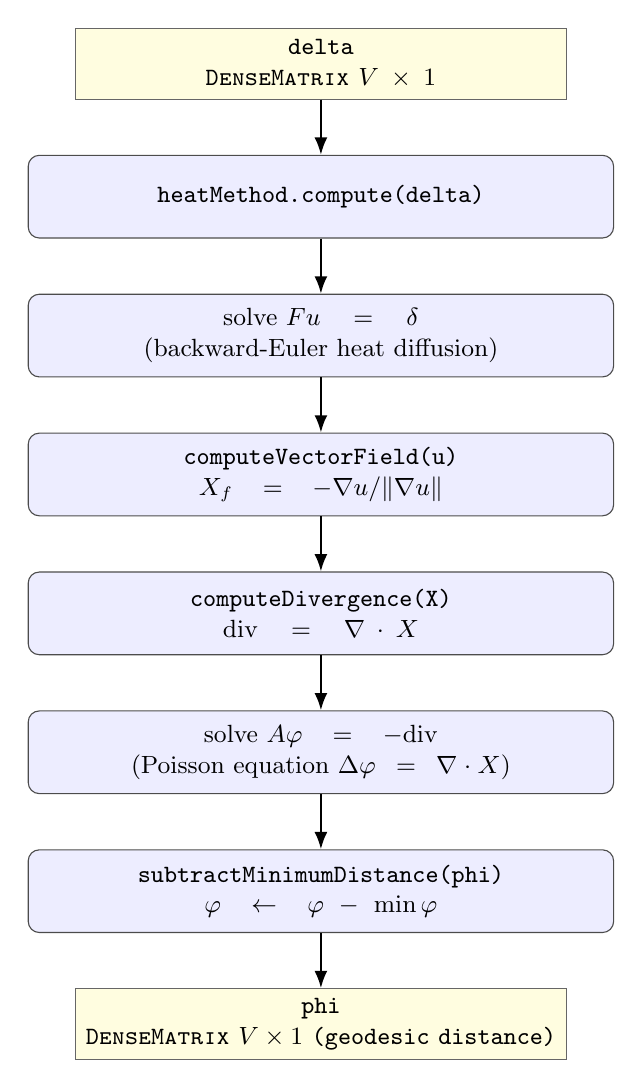
\begin{tikzpicture}[node distance=7mm]
  \node[data] (delta) {\code{delta}\\ \type{DenseMatrix} $V\times1$};
  \node[block, below=of delta] (compute) {\func{heatMethod.compute(delta)}};
  \node[block, below=of compute] (u) {solve $Fu=\delta$ \\ (backward-Euler heat diffusion)};
  \node[block, below=of u] (vf) {\func{computeVectorField(u)}\\ $X_f=-\nabla u/\lVert\nabla u\rVert$};
  \node[block, below=of vf] (div) {\func{computeDivergence(X)}\\ $\mathrm{div} = \nabla\!\cdot\!X$};
  \node[block, below=of div] (poisson) {solve $A\varphi=-\mathrm{div}$\\ (Poisson equation $\Delta\varphi=\nabla\!\cdot\!X$)};
  \node[block, below=of poisson] (shift) {\func{subtractMinimumDistance(phi)}\\ $\varphi \leftarrow \varphi-\min\varphi$};
  \node[data, below=of shift] (phi) {\code{phi}\\ \type{DenseMatrix} $V\times1$ (geodesic distance)};

  \draw[arrowline] (delta) -- (compute);
  \draw[arrowline] (compute) -- (u);
  \draw[arrowline] (u) -- (vf);
  \draw[arrowline] (vf) -- (div);
  \draw[arrowline] (div) -- (poisson);
  \draw[arrowline] (poisson) -- (shift);
  \draw[arrowline] (shift) -- (phi);
\end{tikzpicture}
\end{center}

\subsection{\func{HeatMethod} constructor --- precomputation}
\label{sec:heatmethod-ctor}
\textbf{Input:} \code{geometry} : \type{gpGeometry}.\\
\textbf{Output (new object):} \code{this} : \type{HeatMethod}, exposing
\code{vertexIndex}, \code{A} (\type{SparseMatrix} $V\times V$), \code{F}
(\type{SparseMatrix} $V\times V$).

\begin{lstlisting}
let t = Math.pow(geometry.meanEdgeLength(), 2);
let M = geometry.massMatrix(this.vertexIndex);
this.A = geometry.laplaceMatrix(this.vertexIndex);
this.F = M.plus(this.A.timesReal(t));
\end{lstlisting}

\paragraph{The time step $t$.} $t = \bar\ell^{\,2}$, where $\bar\ell$ is the mean edge
length. Squaring a length gives an area-like quantity, matching the units of the
Laplacian's eigenvalues; this is the standard heuristic from the original heat-method paper
for picking ``a brief period of time'' to diffuse heat --- long enough to smooth out
discretization noise, short enough that heat has not yet ``wrapped around'' the surface (a
requirement for the short-time approximation the method relies on).

\paragraph{The mass matrix $M$ (\func{geometry.massMatrix}).} A diagonal $V\times V$
matrix where $M_{ii} = A_i$ is vertex $i$'s \emph{barycentric dual area} --- one third of
the area of every triangle touching it:
\[
  M_{ii} \;=\; \sum_{f \ni i} \frac{\mathrm{area}(f)}{3}.
\]
Intuitively, $M$ distributes each triangle's area evenly onto its three corners, so that
$M$ acts like a lumped mass in the discrete heat equation, exactly as the mass matrix does
in a finite-element method.

\paragraph{The Laplace matrix $A$ (\func{geometry.laplaceMatrix}).} The classic
\emph{cotangent Laplacian}, but sign-flipped to be positive semidefinite (the code's doc
comment calls this out explicitly: the true Laplace--Beltrami operator is negative
semidefinite, so every off-diagonal weight is stored negated relative to the usual
convention). For vertex $i$ with neighbors $j$:
\[
  A_{ij} = -\frac{\cot\alpha_{ij}+\cot\beta_{ij}}{2}\ \ (j\ne i),
  \qquad
  A_{ii} = \varepsilon + \sum_{j\sim i}\frac{\cot\alpha_{ij}+\cot\beta_{ij}}{2},
\]
where $\alpha_{ij},\beta_{ij}$ are the two angles opposite edge $(i,j)$ in its two incident
triangles, and $\varepsilon=10^{-8}$ is added purely for numerical stability (so $A$ is
strictly positive definite and admits a Cholesky factorization even on meshes with a
non-trivial null space). With this sign convention $A \approx -\Delta$, i.e.\ $A$ plays the
role of the \emph{negative} Laplace--Beltrami operator.

\paragraph{The flow operator $F$.} $F = M + tA$. This single sparse matrix is exactly the
linear system matrix that falls out of discretizing the heat equation
$\partial u/\partial t=\Delta u$ with one \emph{implicit (backward Euler)} step of size $t$:
\[
  M\,\frac{u-u_0}{t} = -A u
  \quad\Longleftrightarrow\quad
  (M + tA)\,u = M u_0.
\]
Backward Euler is used (instead of the simpler forward Euler) because it is unconditionally
stable --- forward Euler on a stiff operator like the cotan Laplacian would require an
absurdly small $t$ to avoid blowing up, whereas implicit Euler stays stable for the fairly
large $t=\bar\ell^2$ chosen above. $F$ is built once per mesh, in the constructor, precisely
because $t$, $M$, and $A$ never change between clicks --- only the right-hand side does.

\subsection{\func{heatMethod.compute(delta)} --- the three-step algorithm}
\label{sec:compute}
\textbf{Input:} \code{delta} : \type{DenseMatrix} $V\times1$ (the discrete source
indicator $\delta$ from Section~\ref{sec:foundation}).\\
\textbf{Output (new object):} \code{phi} : \type{DenseMatrix} $V\times1$, the geodesic
distance estimate $\varphi_i\ge0$ at every vertex.

\begin{lstlisting}
compute(delta) {
  let llt = this.F.chol();
  let u = llt.solvePositiveDefinite(delta);

  let X = this.computeVectorField(u);
  let div = this.computeDivergence(X);

  llt = this.A.chol();
  let phi = llt.solvePositiveDefinite(div.negated());

  this.subtractMinimumDistance(phi);
  return phi;
}
\end{lstlisting}

This is the heat method in exactly three steps, matching Crane, Weischedel \& Wardetzky's
``Geodesics in Heat'' algorithm:

\begin{enumerate}[leftmargin=1.6em]
\item \textbf{Diffuse heat briefly.} \code{this.F.chol()} $\to$ \textbf{new object}
  \code{llt} : \type{Cholesky}, a \emph{sparse Cholesky factorization} $F = LL^{\top}$. A
  Cholesky factorization is the standard way to solve a symmetric positive-definite linear
  system: instead of an expensive general \code{solve}, we factor $F$ once into a lower
  triangular $L$ so that $Fu=\delta \Leftrightarrow LL^{\top}u=\delta$ can be solved by two
  cheap triangular solves (forward-substitute for $y$ in $Ly=\delta$, then
  back-substitute for $u$ in $L^{\top}u=y$). \code{llt.solvePositiveDefinite(delta)} $\to$
  \textbf{new object} \code{u} : \type{DenseMatrix} $V\times1$, solving
  \[
    F u = \delta \quad\Longleftrightarrow\quad (M+tA)\,u=\delta .
  \]
  Conceptually: dump a unit amount of heat at each source vertex ($\delta$) and let it
  diffuse across the surface for time $t$; $u$ is the resulting temperature at every
  vertex. Heat spreads out fastest along the surface in the directions of least
  resistance --- which, for very short times, are exactly the directions of shortest path.

\item \textbf{Extract the direction of steepest descent.} \code{computeVectorField(u)} $\to$
  \textbf{new object} \code{X} : a plain JS dictionary (hash map) $\{\type{Face}\to
  \type{Vector}\}$ (not a matrix type from the library --- just an object keyed by face
  references). See Section~\ref{sec:vectorfield}. This turns the scalar heat field $u$ into
  a per-triangle unit vector field $X\approx -\nabla u/\lVert\nabla u\rVert$: at every
  point, heat flows \emph{away} from the source, so $-\nabla u$ points \emph{toward} the
  source's antipode --- i.e., along the direction distance should increase.

\item \textbf{Find a distance field whose gradient matches $X$.} \code{computeDivergence(X)}
  $\to$ \textbf{new object} \code{div} : \type{DenseMatrix} $V\times1$; see
  Section~\ref{sec:divergence}. Then a second Cholesky factorization is built, this time of
  \code{this.A} (the Laplacian by itself, without the mass/time terms), and used to solve
  the discrete \emph{Poisson equation}
  \[
    \Delta \varphi = \nabla\!\cdot\! X
    \quad\text{discretely}\quad
    A\,\varphi = -\,\mathrm{div},
  \]
  (the sign flips because, as noted above, $A\approx-\Delta$). Solving a Poisson equation
  here means: find the scalar field $\varphi$ whose gradient best matches the vector field
  $X$ in a least-squares sense. Because $X$ was built to point in the direction of
  increasing distance, the $\varphi$ that solves this system is (up to an additive
  constant) the geodesic distance function itself.

\item \textbf{Fix the additive constant.} \func{subtractMinimumDistance(phi)}
  (Section~\ref{sec:submin}) shifts every entry of \code{phi} down by $\min_i\varphi_i$, since
  a Poisson solve only pins down $\varphi$ up to a constant offset, and we want the source
  vertex itself to read a distance of $0$.
\end{enumerate}

\subsection{\func{computeVectorField(u)} --- discrete gradient, per face}
\label{sec:vectorfield}
\textbf{Input:} \code{u} : \type{DenseMatrix} $V\times1$.\\
\textbf{Output (new object):} \code{X} : $\{\type{Face}\to\type{Vector}\}$.

\begin{lstlisting}
computeVectorField(u) {
  let X = {};
  for (let f of this.geometry.mesh.faces) {
    let normal = this.geometry.faceNormal(f);
    let area = this.geometry.area(f);
    let gradU = new Vector();
    for (let h of f.adjacentHalfedges()) {
      let i = this.vertexIndex[h.prev.vertex];
      let ui = u.get(i, 0);
      let ei = this.geometry.vector(h);
      gradU.incrementBy(normal.cross(ei).times(ui));
    }
    gradU.divideBy(2 * area);
    gradU.normalize();
    X[f] = gradU.negated();
  }
  return X;
}
\end{lstlisting}

For a flat triangle $f$ with unit normal $N$, area $\mathrm{area}(f)$, and vertices with
values $u_1,u_2,u_3$, the gradient of the (linearly-interpolated) function $u$ restricted to
that triangle has the closed form
\[
  \nabla u\big|_f \;=\; \frac{1}{2\,\mathrm{area}(f)}\sum_{i=1}^{3} u_i \,\big(N \times \mathbf{e}_i\big),
\]
where $\mathbf{e}_i$ is the edge vector \emph{opposite} vertex $i$ (running along the
halfedge whose \code{.prev.vertex} is $i$, per the code's indexing), oriented consistently
with the face winding. The loop above accumulates exactly this sum, one halfedge $h$ at a
time (\code{normal.cross(ei).times(ui)} for each corner), divides by $2\,\mathrm{area}(f)$,
then normalizes to a unit vector and negates it:
\[
  X_f \;=\; -\,\frac{\nabla u|_f}{\lVert \nabla u|_f\rVert}.
\]
Only the \emph{direction} of $X$ is kept (its magnitude is discarded by
\code{.normalize()}) --- the heat method only needs to know \emph{which way} distance
increases at each triangle, not how fast $u$ changed there.

\subsection{\func{computeDivergence(X)} --- discrete divergence, per vertex}
\label{sec:divergence}
\textbf{Input:} \code{X} : $\{\type{Face}\to\type{Vector}\}$.\\
\textbf{Output (new object):} \code{div} : \type{DenseMatrix} $V\times1$.

\begin{lstlisting}
computeDivergence(X) {
  let div = DenseMatrix.zeros(V, 1);
  for (let v of vertices) {
    let i = this.vertexIndex[v];
    let sum = 0;
    for (let h of v.adjacentHalfedges()) {
      if (!h.onBoundary) {
        let Xj = X[h.face];
        let e1 = this.geometry.vector(h);
        let e2 = this.geometry.vector(h.prev.twin);
        let cotTheta1 = this.geometry.cotan(h);
        let cotTheta2 = this.geometry.cotan(h.prev);
        sum += (cotTheta1 * e1.dot(Xj) + cotTheta2 * e2.dot(Xj));
      }
    }
    div.set(0.5 * sum, i, 0);
  }
  return div;
}
\end{lstlisting}

The standard cotan-weighted divergence of a per-face vector field $X$, evaluated at vertex
$i$, sums a contribution from every triangle touching $i$:
\[
  (\nabla\!\cdot\!X)_i \;=\; \frac12 \sum_{f \ni i}
      \Big(\cot\theta_1\, \mathbf{e}_1\!\cdot\! X_f \;+\; \cot\theta_2\, \mathbf{e}_2\!\cdot\! X_f\Big),
\]
where, for the corner of $f$ at vertex $i$, $\mathbf{e}_1,\mathbf{e}_2$ are the two edges
leaving $i$ and $\theta_1,\theta_2$ are the angles opposite each of them. Geometrically,
divergence measures how much a vector field ``spreads out'' from a point; using the cotan
weights here (rather than plain Euclidean projection) is what makes the discrete operator
compatible with the same cotan Laplacian $A$ used in Section~\ref{sec:heatmethod-ctor} ---
consistency between the discrete gradient/divergence/Laplacian operators is exactly what
makes the Poisson solve in step 3 mathematically sound.

\subsection{\func{subtractMinimumDistance(phi)} --- fix the constant of integration}
\label{sec:submin}
\textbf{Input:} \code{phi} : \type{DenseMatrix} $V\times1$. \textbf{No new object} --- this
function has no return value; it mutates \code{phi}'s existing entries via repeated
\code{phi.set(...)} calls.
\[
  \varphi_i \;\longleftarrow\; \varphi_i - \min_{j} \varphi_j \qquad \text{for every } i.
\]
The Poisson equation $A\varphi=-\mathrm{div}$ only determines $\varphi$ up to an additive
constant (adding the same number to every entry doesn't change any gradient), so nothing in
the linear solve guarantees $\varphi=0$ at the source. This function is the cheap fix:
shift everything down so the smallest value --- which, geometrically, should be at (or very
near) the source vertex --- becomes exactly $0$.

% =====================================================================
\section{Goal B: extraction \& visualization}
\label{sec:goalB}
% =====================================================================

Goal B never touches \code{HeatMethod}'s internals again --- it only consumes the finished
\code{phi} vector (plus the same \code{mesh}/\code{geometry} objects from
Section~\ref{sec:foundation}) and turns numbers into geometry a GPU can rasterize.

\begin{center}
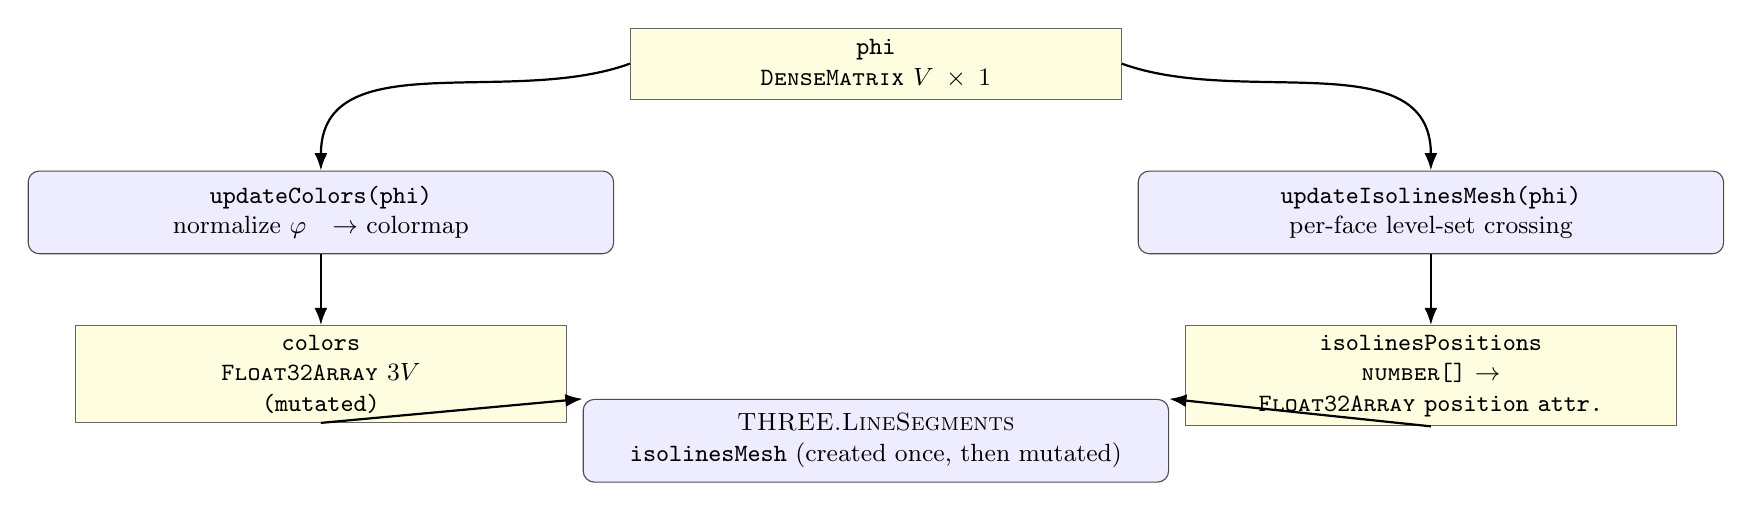
\begin{tikzpicture}[node distance=9mm]
  \node[data] (phi) {\code{phi}\\ \type{DenseMatrix} $V\times1$};
  \node[block, below left=9mm and 2mm of phi] (colors) {\func{updateColors(phi)}\\ normalize $\varphi\to$ colormap};
  \node[block, below right=9mm and 2mm of phi] (iso) {\func{updateIsolinesMesh(phi)}\\ per-face level-set crossing};
  \node[data, below=of colors] (colorbuf) {\code{colors}\\ \type{Float32Array} $3V$\\ (mutated)};
  \node[data, below=of iso] (isopos) {\code{isolinesPositions}\\ \type{number[]} $\to$\\ \type{Float32Array} position attr.};
  \node[block, below=38mm of phi] (mesh3) {\type{THREE.LineSegments}\\ \code{isolinesMesh} (created once, then mutated)};

  \draw[arrowline] (phi.west) to[out=200,in=90] (colors.north);
  \draw[arrowline] (phi.east) to[out=-20,in=90] (iso.north);
  \draw[arrowline] (colors) -- (colorbuf);
  \draw[arrowline] (iso) -- (isopos);
  \draw[arrowline] (colorbuf.south) -- (mesh3.north west);
  \draw[arrowline] (isopos.south) -- (mesh3.north east);
\end{tikzpicture}
\end{center}

\subsection{Prerequisite: \func{initThreeMesh()} builds the drawable mesh}
\label{sec:threemesh}
\textbf{Input:} none (reads outer-scope \code{mesh}, \code{geometry}). \textbf{New objects:}
\code{threeGeometry} : \type{THREE.BufferGeometry}; \code{threeMesh} :
\type{THREE.Mesh}; plus the flat typed arrays \code{positions}, \code{normals},
\code{colors} : \type{Float32Array} of length $3V$, and \code{indices} :
\type{Uint32Array} of length $3F$.

This is ordinary Three.js scaffolding, not heat-method math: for every vertex $v$ with
index $i$ it copies \code{geometry.positions[v]} and
\code{geometry.vertexNormalEquallyWeighted(v)} into flat position/normal buffers at offset
$3i$, and initializes every vertex's color to a flat orange. For every face it writes the
three corner indices into \code{indices}. These three buffers
(\code{positions}/\code{normals}/\code{colors}) are attached to \code{threeGeometry} as
\code{BufferAttribute}s. \textbf{The important detail for Goal B:} \code{colors} is kept as
a live outer-scope array, so \func{updateColors} (below) can overwrite it in place and just
flag \code{threeGeometry.attributes.color.needsUpdate = true} rather than rebuilding the
mesh.

\subsection{\func{updateColors(phi)} --- scalar field $\to$ vertex color}
\textbf{Input:} \code{phi} : \type{DenseMatrix} $V\times1$, or \code{undefined} (no active
sources). \textbf{No new object returned} --- mutates the shared \code{colors}
\type{Float32Array} and flips \code{threeGeometry.attributes.color.needsUpdate}.

\begin{lstlisting}
function updateColors(phi = undefined) {
  maxPhi = phi ? Math.max(...vertices.map(v => phi.get(v.index, 0)), 0) : 0.0;
  for (let v of mesh.vertices) {
    let i = v.index;
    let color = phi
      ? colormap(maxPhi - phi.get(i, 0), 0, maxPhi, hot)
      : ORANGE;
    colors[3*i+0] = color.x; colors[3*i+1] = color.y; colors[3*i+2] = color.z;
  }
  threeGeometry.attributes.color.needsUpdate = true;
}
\end{lstlisting}
(shown slightly condensed; the actual loop finds \code{maxPhi} with an explicit \code{for})

First it computes $\varphi_{\max} = \max_i \varphi_i$. Then every vertex's color is set by
\[
  c_i \;=\; \mathrm{colormap}\!\big(\varphi_{\max}-\varphi_i,\ \ 0,\ \ \varphi_{\max},\ \ \texttt{hot}\big),
\]
i.e.\ the color ramp is driven by $\varphi_{\max}-\varphi_i$ rather than $\varphi_i$
directly: vertices \emph{close} to a source (small $\varphi_i$) get a value \emph{near}
$\varphi_{\max}$, and the ``hot'' colormap paints high values bright --- so sources glow
and distance fades to dark outward. This is pure linear remapping of a scalar into a
lookup-table color, unrelated to differential geometry; it is the last step before the GPU
ever sees the distance field.

\subsection{Source-marker bookkeeping: \func{initThreeSphereMesh} / \func{deleteThreeSphereMesh}}
Both take a \code{v} : \type{Vertex} and return a \type{boolean}. They do not touch
\code{delta} or \code{phi} themselves, but their boolean return value is what
\func{computeDistance} (Section~\ref{sec:bridge}) uses to decide whether $\delta$ actually
changed:
\begin{itemize}[leftmargin=1.6em]
\item \func{initThreeSphereMesh(v)}: if vertex \code{v} has no marker sphere yet, creates
  \textbf{new object} \code{threeSphereMesh} : \type{THREE.Mesh} (a small sphere) at
  \code{geometry.positions[v]}, adds it to \code{scene}, and records it in the
  \code{threeSphereMap} : \type{Map}$\langle$\code{index}, \type{THREE.Mesh}$\rangle$.
  Returns \code{true} only the first time a given vertex is marked (idempotent on repeat
  clicks).
\item \func{deleteThreeSphereMesh(v)}: the inverse --- removes \code{v}'s sphere from
  \code{scene} and from \code{threeSphereMap} if present, returning \code{true} iff a
  sphere actually existed to remove.
\end{itemize}

\subsection{\func{updateIsolinesMesh(phi)} --- level-set extraction}
\label{sec:isolines}
\textbf{Input:} \code{phi} : \type{DenseMatrix} $V\times1$. \textbf{New object (lazily,
once):} \code{isolinesMesh} : \type{THREE.LineSegments} with a fresh
\type{THREE.BufferGeometry} and \type{THREE.LineBasicMaterial}, created only the first time
this is called; every subsequent call \textbf{mutates} the existing mesh by replacing its
\code{position} attribute.

\begin{lstlisting}
let distBetweenLines = maxPhi / 20;
for (let f of mesh.faces) {
  let segment = [];
  for (let h of f.adjacentHalfedges()) {
    let v1 = h.vertex, v2 = h.twin.vertex;
    let i = heatMethod.vertexIndex[v1], j = heatMethod.vertexIndex[v2];
    let region1 = Math.floor(phi.get(i, 0) / distBetweenLines);
    let region2 = Math.floor(phi.get(j, 0) / distBetweenLines);
    if (region1 !== region2) {
      let lambda = /* fraction along edge where an isoline crosses */;
      let p = p1.plus(p2.minus(p1).times(lambda));
      segment.push(p);
    }
  }
  if (segment.length === 2) { /* push segment[0], segment[1] into isolinesPositions */ }
}
isolinesMesh.geometry.addAttribute("position", new THREE.BufferAttribute(new Float32Array(isolinesPositions), 3));
\end{lstlisting}

This is a per-triangle marching-squares-style contouring pass. First, the distance range
$[0,\varphi_{\max}]$ is sliced into 20 equal-width \emph{bands} of width
$d = \varphi_{\max}/20$. Every vertex is assigned a band index
\[
  \mathrm{region}(x) \;=\; \left\lfloor \frac{\varphi_x}{d} \right\rfloor .
\]
For each triangle edge (halfedge $h$, endpoints $v_1,v_2$ with distances $\varphi_i,
\varphi_j$): if the two endpoints fall in \emph{different} bands
($\mathrm{region}_1\ne\mathrm{region}_2$), an isoline boundary must cross that edge
somewhere. Since $\varphi$ is linearly interpolated along the edge, the crossing point is
found by solving for the parameter $\lambda\in[0,1]$ at which the interpolated value hits
the band boundary $k\,d$ (where $k=\max(\mathrm{region}_1,\mathrm{region}_2)$ is whichever
band boundary lies between the two endpoints):
\[
  \varphi_i + \lambda(\varphi_j-\varphi_i) = k\,d
  \quad\Longrightarrow\quad
  \lambda = \frac{k\,d - \varphi_i}{\varphi_j - \varphi_i},
\]
and the corresponding 3D point is the same linear interpolation applied to the endpoint
\emph{positions} rather than their distances:
\[
  \mathbf{p} \;=\; \mathbf{p}_1 + \lambda\,(\mathbf{p}_2-\mathbf{p}_1).
\]
A single triangle has three edges; generically exactly two of them cross a given band
boundary (the isoline enters through one edge and exits through another), which is exactly
the \code{segment.length === 2} check --- those two crossing points become one line segment
of the isolines mesh. (This is a simplified, single-crossing-per-triangle version of
marching squares: it does not attempt to draw more than one isoline through the same
triangle, which is why 20 evenly spaced bands rather than an adaptive/arbitrary set are
used --- with reasonably fine triangles relative to the distance gradient, at most one band
boundary per triangle is the common case.) Finally all segment endpoints, flattened to
\code{[x,y,z,x,y,z,\ldots]}, become the new \code{position} \code{BufferAttribute} on
\code{isolinesMesh}, which is what actually gets rasterized as black contour lines over the
colored surface.

% =====================================================================
\section{The bridge: \func{computeDistance(v)}}
\label{sec:bridge}
% =====================================================================

\func{computeDistance(v)} is the only place Goal A and Goal B are called back to back; it
is triggered by \func{pick()} $\to$ \func{onMouseClick()} whenever the user clicks (or
shift-clicks) a vertex.

\begin{lstlisting}
function computeDistance(v) {
  let compute = false;
  let i = heatMethod.vertexIndex[v];
  if (!shiftClick) {
    selectedVertex = v;
    if (initThreeSphereMesh(v)) { delta.set(1, i, 0); compute = true; }
  } else {
    if (deleteThreeSphereMesh(v)) {
      delta.set(0, i, 0); compute = true;
      if (selectedVertex === v) selectedVertex = undefined;
    }
  }

  if (compute) {
    let phi = delta.sum() > 0 ? heatMethod.compute(delta) : undefined;
    updateColors(phi);
    if (phi) {
      updateIsolinesMesh(phi);
      if (!scene.children.includes(isolinesMesh)) scene.add(isolinesMesh);
    } else {
      scene.remove(isolinesMesh);
    }
    memoryManager.deleteExcept([delta, heatMethod.A, heatMethod.F]);
  }
}
\end{lstlisting}

\begin{enumerate}[leftmargin=1.6em]
\item \textbf{Mutate $\delta$ (input to Goal A).} A plain click sets $\delta_i \leftarrow 1$
  (add vertex $i$ as a heat source) \emph{only if} a new marker sphere was actually created
  (\func{initThreeSphereMesh} returning \code{true} guards against double-adding an
  already-selected vertex). A shift-click sets $\delta_i \leftarrow 0$ (remove it as a
  source) only if a marker sphere actually existed to delete. Either way, the boolean
  \code{compute} tracks whether $\delta$ really changed --- \emph{clicking empty space or an
  already-selected vertex does no work at all.}
\item \textbf{Run Goal A, conditionally.} $\varphi$ is only recomputed
  (\code{heatMethod.compute(delta)}) if \emph{some} source is still active
  (\code{delta.sum() > 0}); if the user has just removed the last source, \code{phi} is left
  \code{undefined} instead of solving a degenerate all-zero system.
\item \textbf{Run Goal B, always (with or without $\varphi$).}
  \func{updateColors(phi)} is called unconditionally --- passing \code{undefined} makes it
  fall back to flat orange (Section~\ref{sec:goalB}). \func{updateIsolinesMesh(phi)} and the
  isolines mesh's presence in \code{scene} are only touched when \code{phi} exists.
\item \textbf{Free WASM heap memory.} \code{delta}, \code{heatMethod.A}, and
  \code{heatMethod.F} live in the emscripten/WASM linear-memory heap (see the
  \type{SparseMatrix}/\type{DenseMatrix} constructors, which register every instance with a
  global \code{memoryManager}) and are \emph{not} garbage-collected by the JS engine.
  \code{memoryManager.deleteExcept([...])} frees every other WASM-backed object allocated
  during this call --- the Cholesky factorizations, \code{u}, \code{div}, and the discarded
  \code{phi} from a previous click --- while explicitly keeping the three matrices that must
  survive until the \emph{next} click. This bookkeeping has no DDG meaning of its own, but
  it is why the pipeline can be re-run every click without leaking memory: each call to
  Goal A allocates a handful of new \type{DenseMatrix}/\type{Cholesky} objects, and this line
  is where they get reclaimed.
\end{enumerate}

% =====================================================================
\section{Summary table}
% =====================================================================

\begin{center}
\small
\renewcommand{\arraystretch}{1.3}
\begin{tabular}{@{}p{3.4cm}p{4.6cm}p{4.9cm}@{}}
\toprule
\textbf{Function} & \textbf{Input $\to$ Output / mutation} & \textbf{Role} \\
\midrule
\multicolumn{3}{@{}l}{\textit{Foundation (Section~\ref{sec:foundation})}} \\
\func{initMesh} & OBJ text $\to$ mutates \code{mesh},\code{geometry},\code{delta},\code{heatMethod} & load \& normalize mesh, allocate $\delta=\vec0$ \\
\func{Mesh\#build} & polygon soup $\to$ \type{boolean}, mutates \code{mesh} & build halfedge combinatorics \\
\func{new Geometry} & mesh, positions $\to$ \type{gpGeometry} & store \& normalize vertex positions \\
\midrule
\multicolumn{3}{@{}l}{\textit{Goal A --- numerical core (Section~\ref{sec:goalA})}} \\
\func{HeatMethod ctor} & \type{gpGeometry} $\to$ \type{HeatMethod} & precompute $t,M,A,F$ \\
\func{compute} & $\delta$ $\to$ $\varphi$ (new \type{DenseMatrix}) & full 3-step heat method \\
\func{computeVectorField} & $u$ $\to$ $\{f\to X_f\}$ & per-face unit gradient direction \\
\func{computeDivergence} & $X$ $\to$ $\mathrm{div}$ (new \type{DenseMatrix}) & cotan divergence, per vertex \\
\func{subtractMinimumDistance} & $\varphi$ mutated in place & pin additive constant to 0 \\
\midrule
\multicolumn{3}{@{}l}{\textit{Goal B --- extraction \& visualization (Section~\ref{sec:goalB})}} \\
\func{initThreeMesh} & mesh, geometry $\to$ \type{THREE.BufferGeometry}/\type{Mesh} & drawable surface + color/normal buffers \\
\func{updateColors} & $\varphi$ (or none) mutates \code{colors} buffer & distance $\to$ colormap \\
\func{initThreeSphereMesh} & vertex $\to$ \type{boolean}, mutates \code{scene}/\code{threeSphereMap} & add source marker \\
\func{deleteThreeSphereMesh} & vertex $\to$ \type{boolean}, mutates \code{scene}/\code{threeSphereMap} & remove source marker \\
\func{updateIsolinesMesh} & $\varphi$ $\to$ mutates/creates \code{isolinesMesh} & level-set contour extraction \\
\midrule
\func{computeDistance} & clicked vertex $\to$ orchestrates all of the above & bridge: click $\to$ $\delta$ $\to$ Goal A $\to$ Goal B \\
\bottomrule
\end{tabular}
\end{center}

\end{document}
